%-------------- Hardware Description ------------------ %
\section{Implementation}
Overview of the test setup can be seen in FIGURE, Implementation can be divided in three parts
\begin{enumerate}
\item \textbf{Full Spectrum Simulator (FSS):} Which will have the power system model, through which different test conditions will be given
\item \textbf{PMU:} Which will consist of a ADC interfacing board and OMAP-L 137 EVM
\item \textbf{PC:} It will have a Phasor Data Concentrator (PDC), which receives data from the PMU and record it for future analysis.
\end{enumerate}
During the initial phase of the project intention was to use indegenously PMU developed C-DAC but due to the hardware issues and lack of documentation and support, it was decided that a minimalistic PMU will be developed by ourself.

\subsection{Full Spectrum Simulator:}
As per the requirement of the implementation, miniature-Full spectrum Simulator will be used for this purpose. FSS is a card based, multi CPU - parallel processing hardware.It uses TI's MSP430 DSPs as building block. It was developed by IIT Bombay and CDAC for both, offline \& real-time  simulation purposes in Power Electronics and Power Systems.

\begin{figure}[th]
\centering
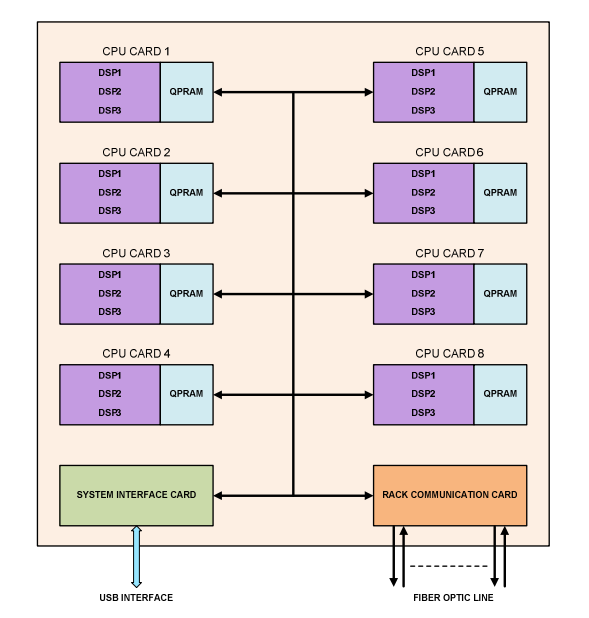
\includegraphics[width=250pt]{fig/FSS_arch.png}
\end{figure}